\documentclass[12pt]{article}

\usepackage[margin=1in]{geometry}
\usepackage{fancyhdr}
\pagestyle{fancy}
\usepackage{amsmath}
\usepackage{amssymb}

% limit to particular location
\usepackage{float}

% graphics
\usepackage{graphicx}
% for subfigures
\usepackage{subcaption}

% better ref links
\usepackage{hyperref}

% footnote in footer
\newcommand{\fancyfootnotetext}[2]{%
  \fancypagestyle{dingens}{%
    \fancyfoot[LO,RE]{\parbox{7cm}{\footnotemark[#1]\footnotesize #2}}%
  }%
  \thispagestyle{dingens}%
}

\lhead{HW1}
\chead{Digital Image Processing}
\rhead{B03902036}


\begin{document}

\section*{Warm-up}
\begin{figure*}[ht!]
    \centering
    \begin{subfigure}[t]{0.3\textwidth}
        \centering
        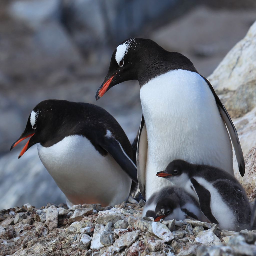
\includegraphics[height=1.5in]{images/I1}
        \caption{sample1.raw ($I_1$)}
    \end{subfigure}%
    ~ 
    \begin{subfigure}[t]{0.3\textwidth}
        \centering
        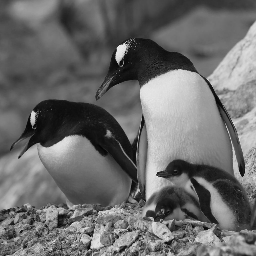
\includegraphics[height=1.5in]{images/I1_gray}
        \caption{Grayscale}
    \end{subfigure}%
    ~
    \begin{subfigure}[t]{0.3\textwidth}
        \centering
        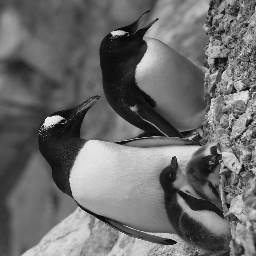
\includegraphics[height=1.5in]{images/B}
        \caption{Diagonally flipped (B)}
    \end{subfigure}
    \caption{Simple manipulations}
\end{figure*}

\section*{Problem 1}
\subsection*{Divide-by-3}
\begin{figure*}[ht!]
    \centering
    \begin{subfigure}[t]{0.3\textwidth}
        \centering
        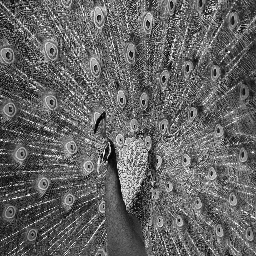
\includegraphics[height=1.5in]{images/I2}
        \caption{sample2.raw ($I_2$)}
    \end{subfigure}%
    ~ 
    \begin{subfigure}[t]{0.7\textwidth}
        \centering
        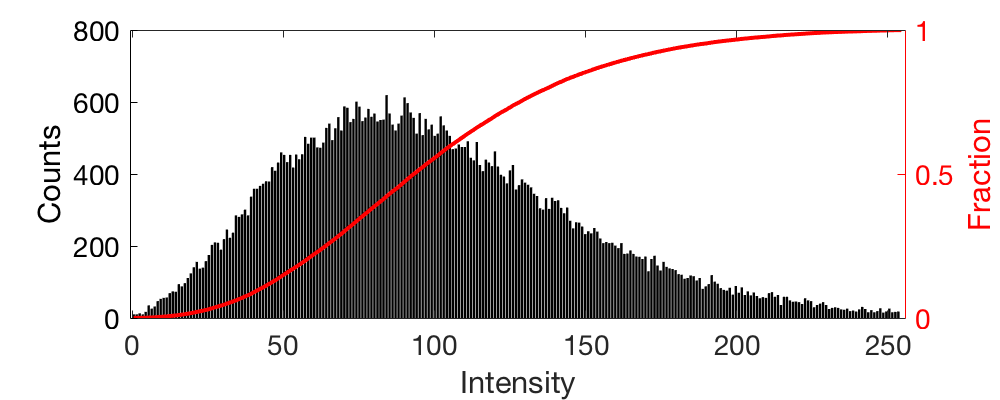
\includegraphics[height=1.5in]{images/I2_histogram}
        \caption{Histogram of $I_2$}
    \end{subfigure}%
    
    \vskip\baselineskip
    \begin{subfigure}[t]{0.3\textwidth}
        \centering
        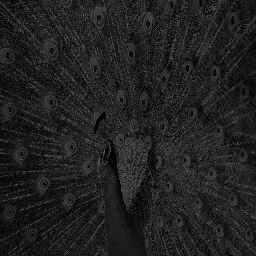
\includegraphics[height=1.5in]{images/D}
        \caption{Brightness decreased (D)}
    \end{subfigure}%
    ~
    \begin{subfigure}[t]{0.7\textwidth}
        \centering
        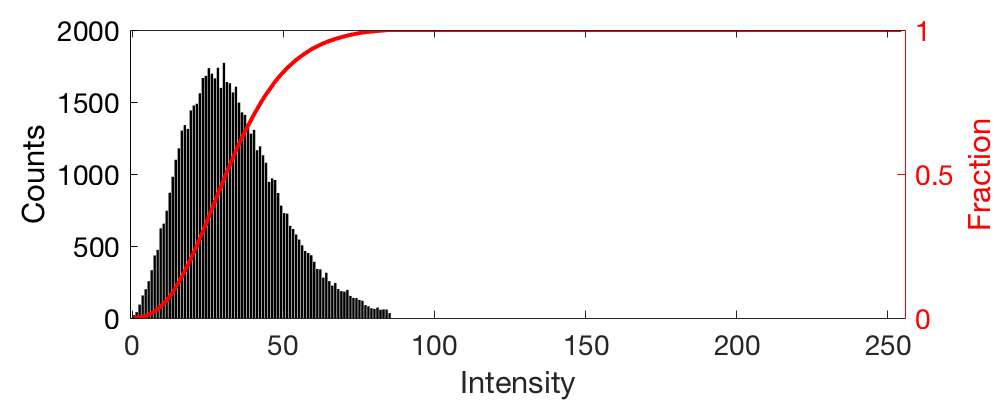
\includegraphics[height=1.5in]{images/D_histogram}
        \caption{Histogram of D}
        \label{fig:D_hist}
    \end{subfigure}%
    ~
    \caption{Histogram after intensity divisions}
    \label{fig:intensity_div}
\end{figure*}
From \autoref{fig:intensity_div}, due to division, all the pixels are accumulated at low intensity portion of the curve, yielding the right-skewed histogram. 
The division also causes pixels to have relatively fewer levels to present their contrast, hence the fraction curve rises in histogram of D.

\subsection*{Histogram equalization}
\begin{figure*}[ht!]
    \centering
    \begin{subfigure}[t]{0.3\textwidth}
        \centering
        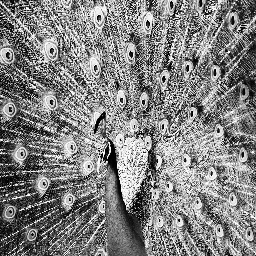
\includegraphics[height=1.5in]{images/H}
        \caption{Global (H)}
    \end{subfigure}%
    ~ 
    \begin{subfigure}[t]{0.7\textwidth}
        \centering
        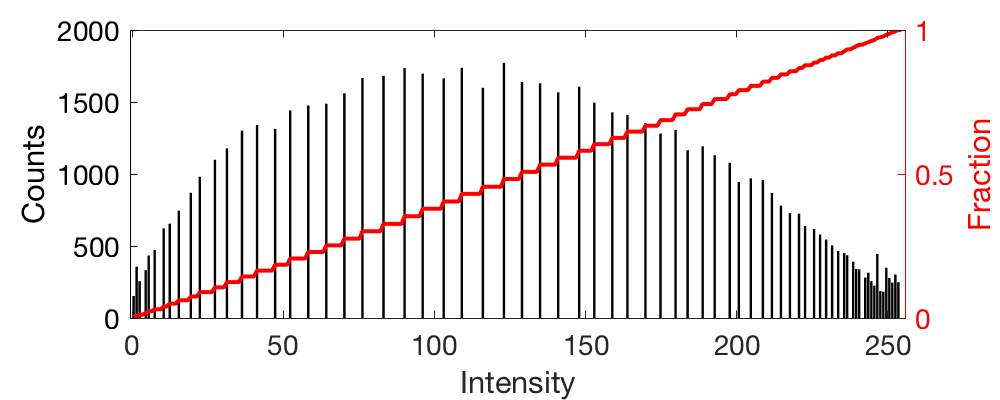
\includegraphics[height=1.5in]{images/H_histogram}
        \caption{Histogram of H}
        \label{fig:H_hist}
    \end{subfigure}%
    
    \vskip\baselineskip
    \begin{subfigure}[t]{0.3\textwidth}
        \centering
        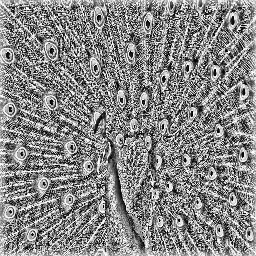
\includegraphics[height=1.5in]{images/L}
        \caption{Local (L), $k=15$}
    \end{subfigure}%
    ~
    \begin{subfigure}[t]{0.7\textwidth}
        \centering
        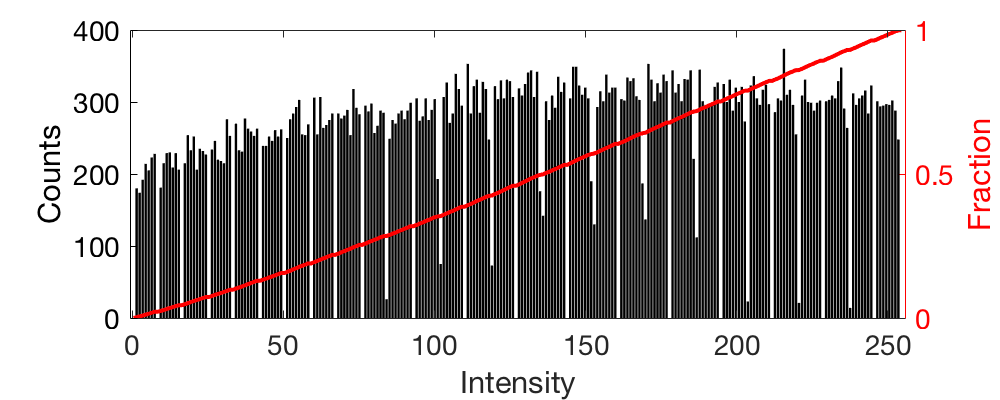
\includegraphics[height=1.5in]{images/L_histogram}
        \caption{Histogram of L}
    \end{subfigure}%
    ~
    \caption{Histogram after histogram equalization}
    \label{fig:histeq}
\end{figure*}
By building a simple transfer function to convert the distribution of pixels in D as uniformly as possible, we have H.
The stretching is visible in its histogram (\autoref{fig:H_hist}) as gaps due to information loss during the division (pixels in similar levels are forced to group as the same one).

Since local histogram equalization only consider intensity distribution in a defined, small region (kernel size is 15), it potentially allows one to visualize more details, but also being prone to background noise.
Hence, while L is visually clear in the orientation of feathers, noise is also visible after zoom-in.
Convolving the equalization filter also allows L to distributes pixels more uniformly, since the transfer function do not have to accommodate for wide intensity variations (globally speaking).

When one compares the result with \autoref{fig:D_hist}, envelope from global histogram equalization highly resemble the envelope of the original image's histogram, which is not visible in the local histogram equalization.

\newpage

\subsection*{Transformations}
\begin{figure*}[ht!]
    \centering
    \begin{subfigure}[t]{0.3\textwidth}
        \centering
        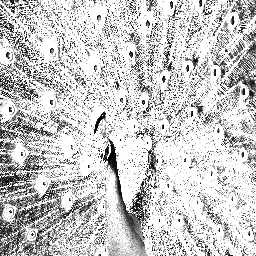
\includegraphics[height=1.5in]{images/Dlog_a2}
        \caption{$y=log_2 (1+2x)$}
        \label{fig:dlog_a2}
    \end{subfigure}%
    ~ 
    \begin{subfigure}[t]{0.7\textwidth}
        \centering
        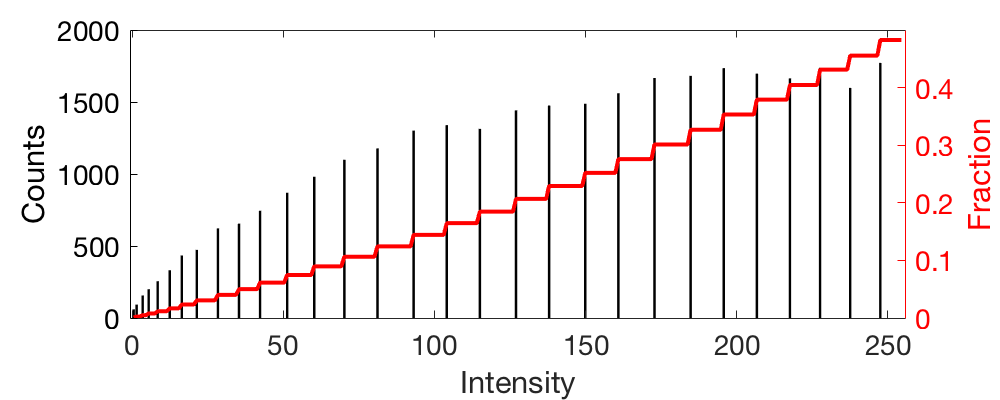
\includegraphics[height=1.5in]{images/Dlog_a2_histogram}
        \caption{Histogram of \autoref{fig:dlog_a2}}
    \end{subfigure}%
    
    \vskip\baselineskip
    \begin{subfigure}[t]{0.3\textwidth}
        \centering
        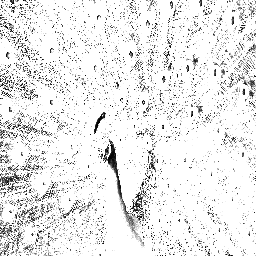
\includegraphics[height=1.5in]{images/Dlog_a5}
        \caption{$y=log_2 (1+5x)$}
        \label{fig:dlog_a5}
    \end{subfigure}%
    ~
    \begin{subfigure}[t]{0.7\textwidth}
        \centering
        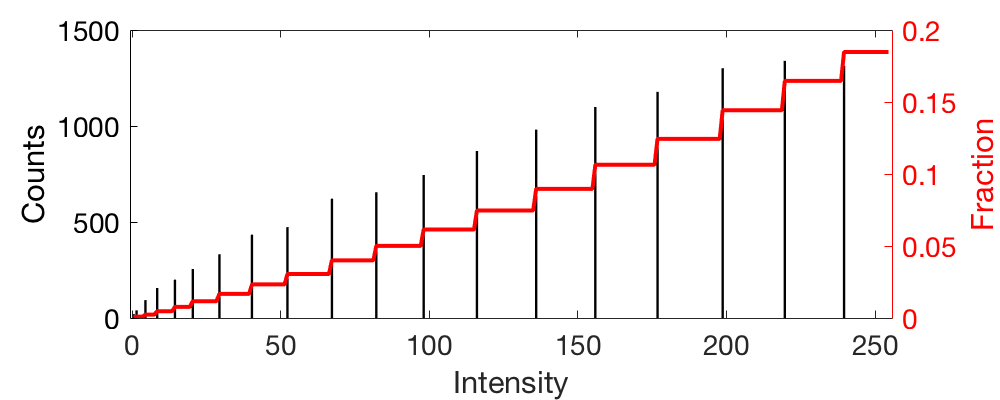
\includegraphics[height=1.5in]{images/Dlog_a5_histogram}
        \caption{Histogram of \autoref{fig:dlog_a5}}
    \end{subfigure}%
    
    \vskip\baselineskip
    \begin{subfigure}[t]{0.3\textwidth}
        \centering
        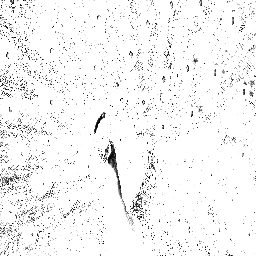
\includegraphics[height=1.5in]{images/Dlog_a10}
        \caption{$y=log_2 (1+10x)$}
        \label{fig:dlog_a10}
    \end{subfigure}%
    ~ 
    \begin{subfigure}[t]{0.7\textwidth}
        \centering
        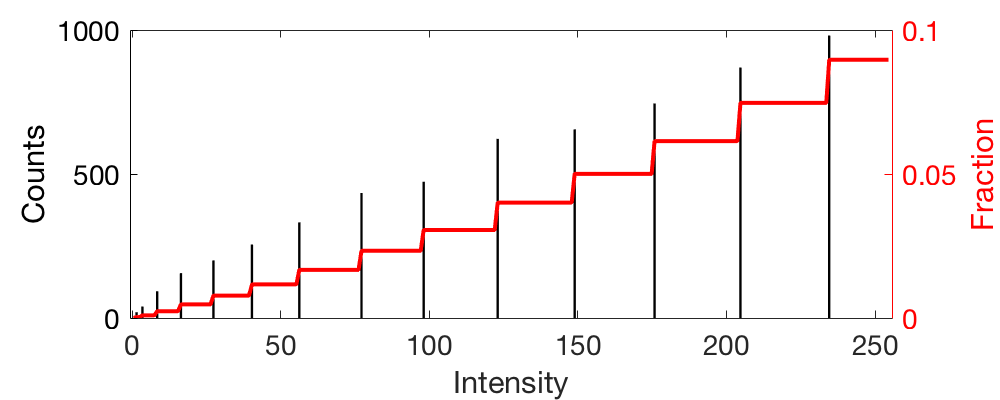
\includegraphics[height=1.5in]{images/Dlog_a10_histogram}
        \caption{Histogram of \autoref{fig:dlog_a10}}
    \end{subfigure}%
    ~
    \caption{$log$ transform}
    \label{fig:log_trans}
\end{figure*}
The logarithm function expend the brighter regions while compress the darker regions.
As the factor increases, it darker regions are push forward to the brighter regions, causing them to get expand faster, this causes the dramatic increase both in gaps and quantities at the right-hand side of the histograms.

\newpage

\begin{figure*}[ht!]
    \centering
    \begin{subfigure}[t]{0.3\textwidth}
        \centering
        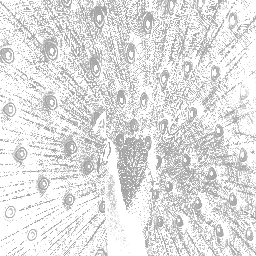
\includegraphics[height=1.5in]{images/Dinvlog_a2}
        \caption{$y=\frac{1}{log_2 (1+2x)}$}
        \label{fig:dinvlog_a2}
    \end{subfigure}%
    ~
    \begin{subfigure}[t]{0.7\textwidth}
        \centering
        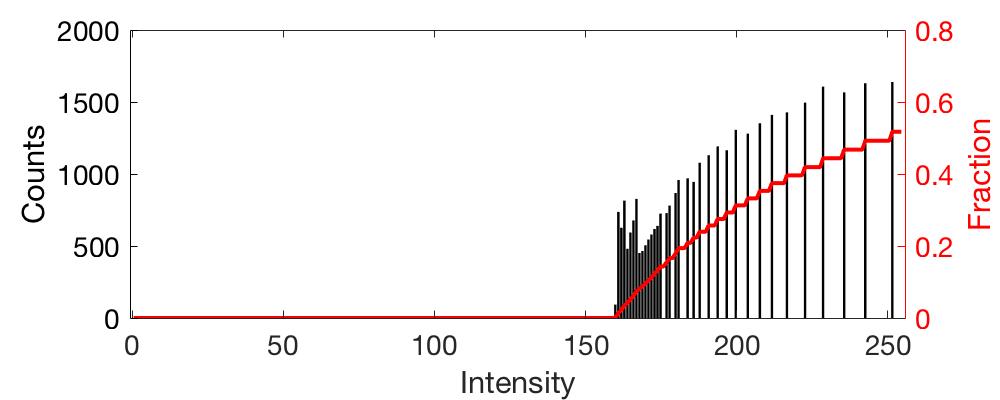
\includegraphics[height=1.5in]{images/Dinvlog_a2_histogram}
        \caption{Histogram of \autoref{fig:dinvlog_a2}}
    \end{subfigure}%
    
    \vskip\baselineskip
    \begin{subfigure}[t]{0.3\textwidth}
        \centering
        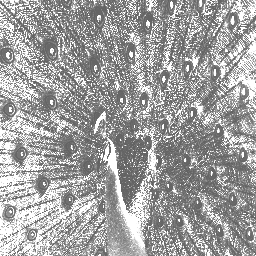
\includegraphics[height=1.5in]{images/Dinvlog_a5}
        \caption{$y=\frac{1}{log_2 (1+5x)}$}
        \label{fig:dinvlog_a5}
    \end{subfigure}%
    ~
    \begin{subfigure}[t]{0.7\textwidth}
        \centering
        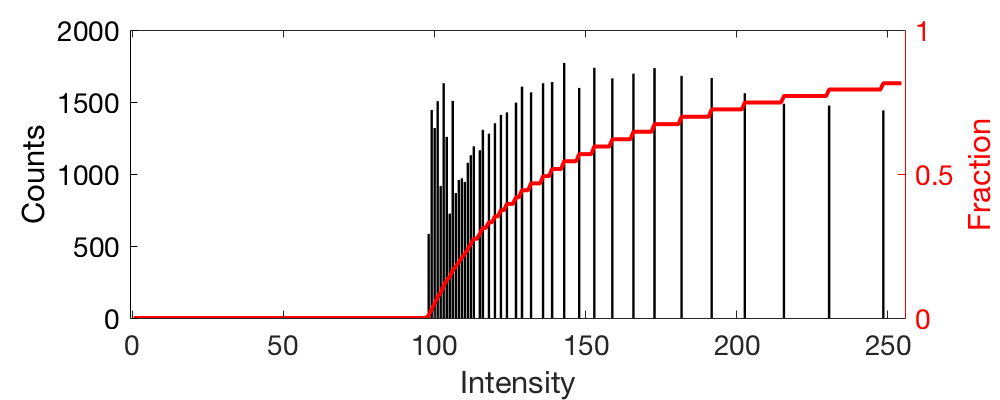
\includegraphics[height=1.5in]{images/Dinvlog_a5_histogram}
        \caption{Histogram of \autoref{fig:dinvlog_a5}}
    \end{subfigure}%
    
    \vskip\baselineskip
    \begin{subfigure}[t]{0.3\textwidth}
        \centering
        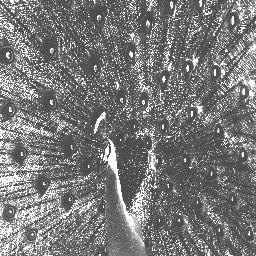
\includegraphics[height=1.5in]{images/Dinvlog_a10}
        \caption{$y=\frac{1}{log_2 (1+10x)}$}
        \label{fig:dinvlog_a10}
    \end{subfigure}%
    ~
    \begin{subfigure}[t]{0.7\textwidth}
        \centering
        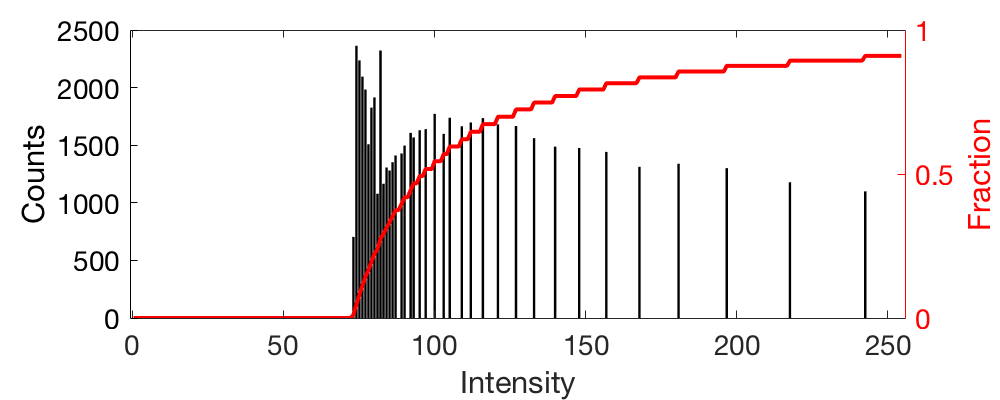
\includegraphics[height=1.5in]{images/Dinvlog_a10_histogram}
	    \caption{Histogram of \autoref{fig:dinvlog_a10}}
    \end{subfigure}%
    \caption{Inverse $log$ transform}
    \label{fig:invlog_trans}
 \end{figure*}
 Inverse of the logarithm function turns all the bright pixels to dark one and vice versa, hence the reversed behavior in the histograms -- in both intensity distribution density and gaps.
  
 \newpage
 
 \begin{figure*}[ht!]
    \centering
    \begin{subfigure}[t]{0.3\textwidth}
        \centering
        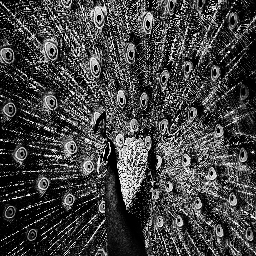
\includegraphics[height=1.5in]{images/Dpow_p3}
        \caption{$y=x^3$}
        \label{fig:dpow_p3}
    \end{subfigure}%
    ~
    \begin{subfigure}[t]{0.7\textwidth}
        \centering
        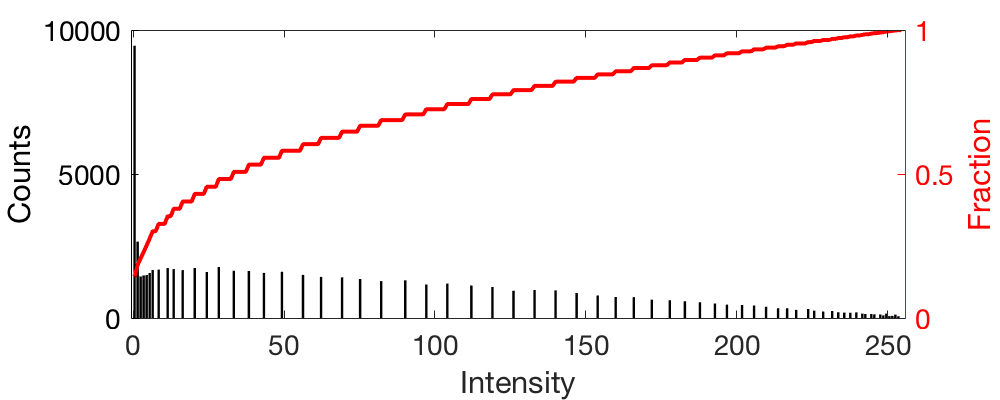
\includegraphics[height=1.5in]{images/Dpow_p3_histogram}
	    \caption{Histogram of \autoref{fig:dpow_p3}}
    \end{subfigure}%
    
    \vskip\baselineskip
    \begin{subfigure}[t]{0.3\textwidth}
        \centering
        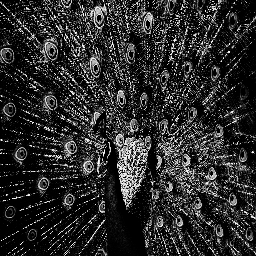
\includegraphics[height=1.5in]{images/Dpow_p5}
        \caption{$y=x^5$}
        \label{fig:dpow_p5}
    \end{subfigure}%
    ~
    \begin{subfigure}[t]{0.7\textwidth}
        \centering
        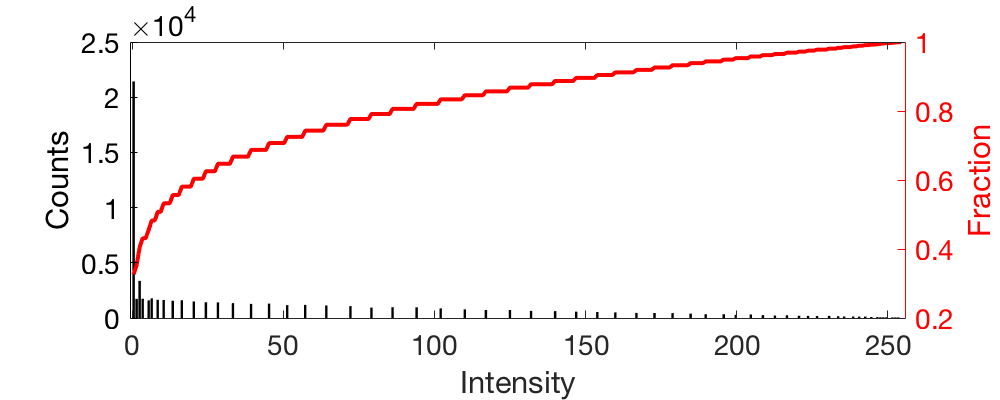
\includegraphics[height=1.5in]{images/Dpow_p5_histogram}
	    \caption{Histogram of \autoref{fig:dpow_p5}}
    \end{subfigure}%
    
    \vskip\baselineskip
    \begin{subfigure}[t]{0.3\textwidth}
        \centering
        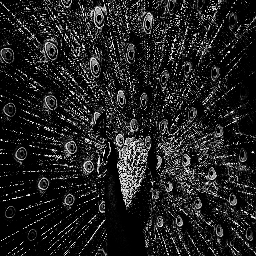
\includegraphics[height=1.5in]{images/Dpow_p7}
        \caption{$y=x^7$}
        \label{fig:dpow_p7}
    \end{subfigure}%
    ~
    \begin{subfigure}[t]{0.7\textwidth}
        \centering
        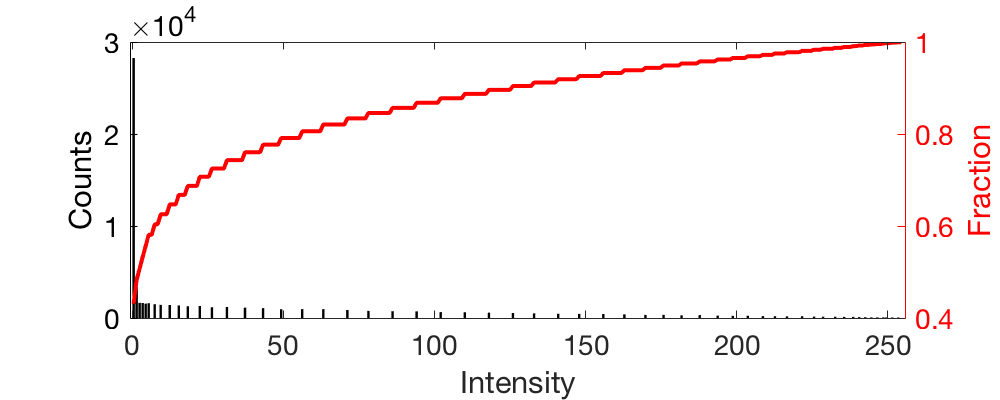
\includegraphics[height=1.5in]{images/Dpow_p7_histogram}
	    \caption{Histogram of \autoref{fig:dpow_p7}}
    \end{subfigure}%
    \caption{Power-law transform}
    \label{fig:pow_trans}
\end{figure*}
Though the power-law behaves similar to the inverse logarithm function, it is continuous at near-zero, therefore, the distribution of the histogram can go all the way to the left hand side instead of having a asymptotic line (\autoref{fig:invlog_trans}).

\newpage

\section*{Problem 2}
\subsection*{Noise generation}
\begin{figure*}[ht!]
    \centering
    \begin{subfigure}[t]{0.3\textwidth}
        \centering
        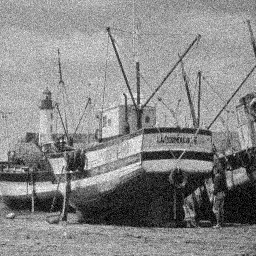
\includegraphics[height=1.5in]{images/G1}
        \caption{$\sigma=16$}
    \end{subfigure}%
    ~ 
    \begin{subfigure}[t]{0.3\textwidth}
        \centering
        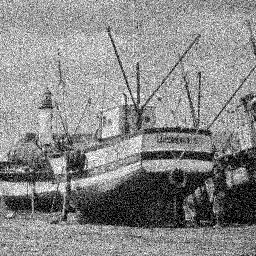
\includegraphics[height=1.5in]{images/G2}
        \caption{$\sigma=32$}
    \end{subfigure}%
    ~
    \caption{Gaussian noise}
\end{figure*}
As $\sigma$ increases, intensity distribution of the noise spreads wider, causing more variety of intensity values to appear in the image.

\begin{figure*}[ht!]
    \centering
    \begin{subfigure}[t]{0.3\textwidth}
        \centering
        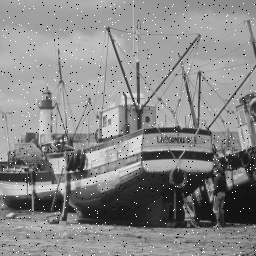
\includegraphics[height=1.5in]{images/S1}
        \caption{threshold $=$ 0.01}
    \end{subfigure}%
    ~ 
    \begin{subfigure}[t]{0.3\textwidth}
        \centering
        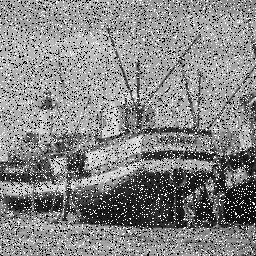
\includegraphics[height=1.5in]{images/S2}
        \caption{threshold $=$ 0.1}
        \label{fig:th_0p1}
    \end{subfigure}%
    ~
    \caption{Salt-n-pepper noise}
\end{figure*}
When the threshold increases, it hints that more sampled random points are allowed to show up as salt or pepper in the image, therefore, we observed that \autoref{fig:th_0p1} has higher density of the impulse noise.

\newpage

\subsection*{Denoise and PSNR}
Since Gaussian noise is uniformly distributed across entire image, using a low-pass filter (LPF) one of the methods to smooth out the flaky effect.
The LPF used has $b=1$, which is effectively an average filter
\begin{equation*}
	H = \frac{1}{m^2} \begin{bmatrix}
	    1_{11} & 1_{12} & \dots  & 1_{1m} \\
	    1_{21} & 1_{22} & \dots  & 1_{2m} \\
	    \vdots & \vdots & \ddots & \vdots \\
	    1_{m1} & 1_{m2} & \dots  & 1_{mm}
	\end{bmatrix}
\end{equation*}
where $m$ denotes the kernel size.

\begin{figure*}[ht!]
    \centering
    \begin{subfigure}[t]{0.3\textwidth}
        \centering
        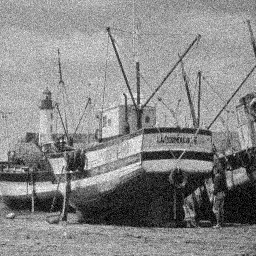
\includegraphics[height=1.5in]{images/G1}
        \caption{Before}
    \end{subfigure}%
    ~ 
    \begin{subfigure}[t]{0.3\textwidth}
        \centering
        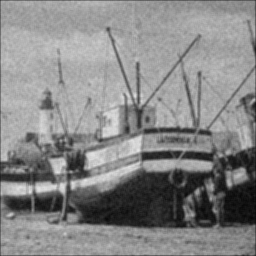
\includegraphics[height=1.5in]{images/Rg}
        \caption{After ($m=3$)}
    \end{subfigure}%
    ~
    \caption{Low-pass filter}
\end{figure*}

If we increase the kernel size ($m$), which is currently minimal, the image only deteriorate further, illustrated in \autoref{fig:g_ksz}, determined by the PSNR.

\begin{figure*}[ht!]
    \centering
    \begin{subfigure}[t]{0.3\textwidth}
        \centering
        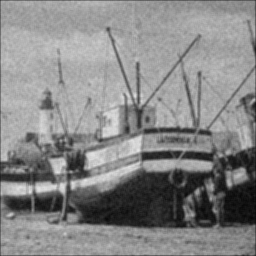
\includegraphics[height=1.5in]{images/Rg}
        \caption{$m=3$, PSNR = 25.9 dB}
    \end{subfigure}%
    ~ 
    \begin{subfigure}[t]{0.3\textwidth}
        \centering
        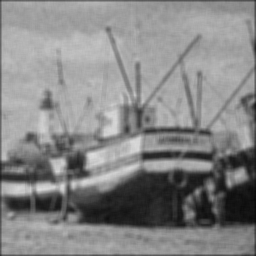
\includegraphics[height=1.5in]{images/Rg_5}
        \caption{$m=5$, PSNR = 23.4 dB}
    \end{subfigure}%
    ~
    \begin{subfigure}[t]{0.3\textwidth}
        \centering
        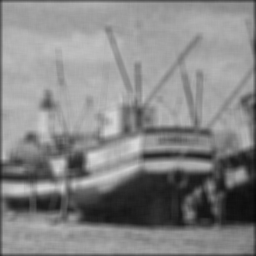
\includegraphics[height=1.5in]{images/Rg_7}
        \caption{$m=7$, PSNR = 21.9 dB}
    \end{subfigure}
    \caption{Different kernel size.}
    \label{fig:g_ksz}
\end{figure*}

In this implementation, images are zero-padded instead of mirror-padded, hence the surrounding of the images will gradually show black boundaries as the kernel size increases.

\newpage

\begin{figure*}[ht!]
    \centering
    \begin{subfigure}[t]{0.3\textwidth}
        \centering
        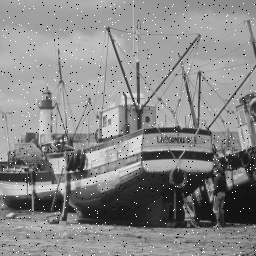
\includegraphics[height=1.5in]{images/S1}
        \caption{Before}
    \end{subfigure}%
    ~ 
    \begin{subfigure}[t]{0.3\textwidth}
        \centering
        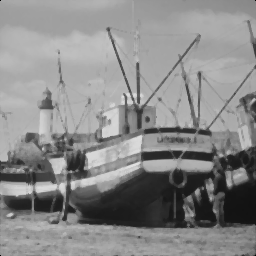
\includegraphics[height=1.5in]{images/Rs}
        \caption{After}
    \end{subfigure}%
    ~
    \caption{Median filter}
\end{figure*}

Since impulse noise are localized to specific regions (in low density), using average filter to smooth them out is an overkill.
The extremity nature of the salt-n-pepper noise makes it an excellent candidate for the median filter, which chooses the most average-behaved intensity to keep, yet, rest of the pixels remain untouched.

\begin{figure*}[ht!]
    \centering
    \begin{subfigure}[t]{0.3\textwidth}
        \centering
        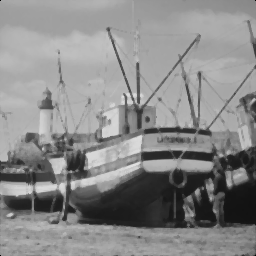
\includegraphics[height=1.5in]{images/Rs}
        \caption{$m=3$, PSNR = 29.1 dB}
    \end{subfigure}%
    ~ 
    \begin{subfigure}[t]{0.3\textwidth}
        \centering
        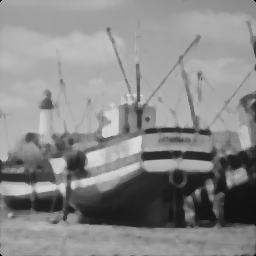
\includegraphics[height=1.5in]{images/Rs_5}
        \caption{$m=5$, PSNR = 25.2 dB}
    \end{subfigure}%
    ~
    \begin{subfigure}[t]{0.3\textwidth}
        \centering
        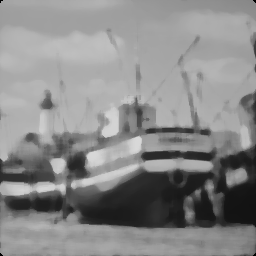
\includegraphics[height=1.5in]{images/Rs_7}
        \caption{$m=7$, PSNR = 23.4 dB}
    \end{subfigure}
    \caption{Different kernel size.}
    \label{fig:s_ksz}
\end{figure*}

Optimal kernel size is still minimal ($m=3$) in this case, determined by the PSNR.

\newpage

\subsection*{Wrinkle removal}
\begin{figure*}[ht!]
    \centering
    \begin{subfigure}[t]{0.3\textwidth}
        \centering
        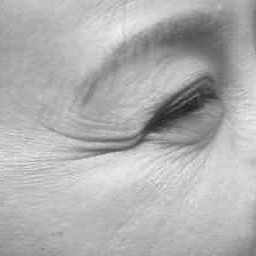
\includegraphics[height=1.5in]{images/I4}
        \caption{Before}
    \end{subfigure}%
    ~ 
    \begin{subfigure}[t]{0.3\textwidth}
        \centering
        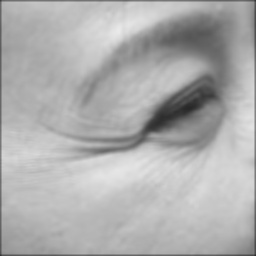
\includegraphics[height=1.5in]{images/smooth}
        \caption{After}
    \end{subfigure}%
\end{figure*}

Using kernel size of 14 to suppress the fine lines, but the mermaid lines will require edge detection for better result \footnotemark[1]\fancyfootnotetext{1}{I have run out of time.}. 

\end{document}
              